% Chapter Template

\chapter{Metodología} % Main chapter title
\label{Chapter2}



%\chapquote{En este capítulo se incluye una breve descripción de distintos proyectos que han
%influenciado el desarrollo de este Trabajo de Fin de Grado. En la sección \ref{sec:automail}
%el proyecto combina Myo, Raspberry Py y Arduino para realizar movimientos simples en una
%prótesis.}

\chapquote{En este segundo capítulo, se hablará de los distintos elementos que
conforman la tesis. En apartado~\ref{sec:introducción2} se dará un breve resumen.
A continuación, el apartado~\ref{sec:tecnologías} hablará tanto de los
componentes software como hardware que han sido utilizados. Por último, el apartado \ref{sec:prótesis-electrónica} muestra el entorno de trabajo real.}

% TODO: http://ieeexplore.ieee.org/xpl/login.jsp?tp=&arnumber=5670617&url=http%3A%2F%2Fieeexplore.ieee.org%2Fxpls%2Fabs_all.jsp%3Farnumber%3D5670617
% TODO: http://ieeexplore.ieee.org/xpl/login.jsp?tp=&arnumber=6361492&url=http%3A%2F%2Fieeexplore.ieee.org%2Fxpls%2Fabs_all.jsp%3Farnumber%3D6361492


\section{Introducción}
\label{sec:introducción2}

%Este capítulo aportará información respecto a cómo se ha elaborado el trabajo.
%El proyecto de esta tesis pretende ser un proyecto, por lo cual se ha requerido
%no solo del estudio e investigación de otros proyectos, sino que se ha tenido
%que desarrollar de forma práctica. Por ello, en el subapartado \ref{sec:tecnologías}
%se explicará algunos recursos utilizados para el desarrollo del proyecto.

%TODO completar con lo que se desarrolle más adelante

Debido a la amplitud del proyecto, en este capítulo se pretende dar un repaso a todas las herramientas utilizadas así como una breve descripción de las mismas y por qué han sido elegidas. Por una parte, en el subapartado \ref{sub:software} se describen las herramientas utilizadas para desarrollar el modelo de aprendizaje que controlará la prótesis, además se incluye una descripción de los programas utilizados para poder imprimir los modelos 3D de la prótesis en la impresora 3D (en \ref{subs:prusa-i3} se describe la impresora utilizada). Por otra parte, el subapartado \ref{sub:hardware}, contiene tanto la descripción de las herramientas físicas utilizadas, es decir, todos los sensores, cotroladores y la propia impresora 3D anteriormente citada. Por último, el apartado \ref{sec:prótesis-electrónica} describe más en profundidad el funcionamiento de la prótesis y sus componentes electrónicos.



\section{Tecnologías}
\label{sec:tecnologías}

En este apartado se aportará información tanto del \textit{software},
subapartado~\ref{sub:software}, como del \textit{hardware}, subapartado~\ref{sub:hardware},
empleado para el desarrollo del proyecto.


\subsection{Software}
\label{sub:software}

La parte \textit{software} del proyecto recae sobre la implementación de algoritmos de
aprendizaje automático y la comunicación entre los diferentes componentes
(descritos en el subapartado~\ref{sub:hardware}). De forma adicional, se
añadirá de forma breve los programas necesarios para la impresión de la prótesis.

%TODO: mencionar python y git como subsubapartado o como párrafo aqui?


\subsubsection{Scikit-learn}
\label{subs:scikit-learn}

%TODO: añadir SVM a los acrónimos

Scikit-learn \cite{scikit-learn} es un módulo de Python que integra un gran
número de algoritmos de aprendizaje automático para problemas de tamaño medio de
clasificación y regresión.

\begin{figure}[htp]
  \centering
    \includegraphics[width=0.4\textwidth]{Chapter2/scikit-learn}
  \caption{Logo de Scikit-learn}
\label{fig:scikit-learn}
\end{figure}

 El módulo cuenta con la librería de C++ LibSVM y
LibLinear para la implementación de SVM y modelos lineales generalizados. Está
construido además sobre \textit{numpy}, que proporciona la estructura base de
los datos y el modelo de parámetros; \textit{Scipy}, que aporta algoritmos
eficientes para álgebra lineal, representación de matrices dispersas y funciones
de estadística básica; y por último \textit{Cython}, un lenguaje que combina
\textit{C} y \textit{Python} para obtener el rendimiento de los lenguajes
compilados, con la sintaxis y las operaciones de un lenguaje de alto nivel como
\textit{Python}.

Como la mayoría del ecosistema Python, Scikit-learn está distribuido mediante
una licencia BSD, lo que permite su uso en proyectos comerciales, que a su vez,
contribuyen a mantener el desarrollo del proyecto. Algunas de las empresas que
usan Scikit-learn son Spotify y Evernote \cite{scikit-learn-empresas}.

Se ha elegido este proyecto para la clasificación de las poses por la versatilidad
y rapidez de desarrollar prototipos, la vigencia y eficiencia de los algoritmos
que implementa. Además aporta en su documentación toda la base matemática y
explicaciones del funcionamiento de los algoritmos, es decir, no solo aporta
información acerca de como usar los algoritmos en Python, sino también su base
teórica.


\subsubsection{Theano}
\label{subs:theano}

\begin{figure}[htp]
  \centering
    \includegraphics[width=0.4\textwidth]{Chapter2/theano}
  \caption{Logo de Theano}
\label{fig:theano}
\end{figure}


Theano es la librería que utilizan como base la mayoría de \textit{frameworks} orientados al \textit{deep learning} 
en \textit{Python} \cite{theano-based-projects}. Su uso permite definir, optimizar y evaluar expresiones matemáticas 
mediante \cite{theano}:

\begin{itemize}

	\item Uso de compiladores como \textit{g++} o \textit{nvcc} para optimizar la velocidad de ejecución.
	\item Diferenciación simbólica para construir grafos simbólicos para computar gradientes automáticamente.
	\item Reconocimiento de (algunas) expresiones numéricas inestables. 
	\item Soporte de operaciones dispersas, tensores y álgebra lineal.
	\item Ejecución en paralelo (SIMD, multinúcleo y multinodo en cluster o distribuido).

\end{itemize}


\subsubsection{Lasagne}
\label{subs:lasagne}

Lasagne es una librería ligera para construir y entrenar redes neuronales en theano de forma simple, transparente (no abstrae las expresiones de Theano) y modular~\cite{lasagne}. Sus principales características son:

\begin{itemize}

	\item Permite implementar redes prealimentadas como redes neuronales convolucionales, redes neuronales recurrentes y combinaciones de cualquier modelo de las redes mencionadas.
	\item Permite arquitecturas de cualquier número de entradas y salidas, incluso clasificadores auxiliares.
	\item Uso de métodos de optimización como \textit{Nesterov momentum}, \textit{RMSprop} y \textit{ADAM}.
	\item Uso de CPU y GPU mediante el uso del compiladore de expresiones de Theano.
\end{itemize}



\subsubsection{Nolearn}
\label{subs:nolearn}

Nolearn \cite{nolearn} es un conjunto de \textit{wrappers} y abstraciones de distintas librerías de redes neuronales (principalmente Lasagne) cuya principal característica, y motivo por el que se ha utilizado en este trabajo, es que todo el código es compatible con \textit{Scikit-learn}. El uso de esta librería permite construir una red neuronal y que sea reconocido como un modelo de \textit{Scikit-learn} pudiendo usar cualquier implementación auxiliar de esta librería como si la red neuronal fuera un modelo nativo.

Para mantener la compatibilidad existen ciertas pautas que se han de seguir para desarrollar las redes neuronales. La implementación puede verse en el apartado \ref{nn-arquitecture}



\subsubsection{Myo-raw}
\label{subs:myo-raw}

Proyecto independiente y libre que aporta una interfaz para poder comunicarse
con el dispositivo EMG Thalmic Myo, mediante la posibilidad de poder escanear
y conectarse al dispositivo más cercano, pudiendo de esta forma, acceder a los
datos de los sensores \cite{myo-raw}.

En concreto, este proyecto incluye los siguientes ficheros \textit{.py}:
\textit{myo\_raw.py} provee el acceso a los datos EMG, mediante la clase
MyoRaw, el cual implementa el protocolo de comunicación con la Myo.
\textit{classify\_myo.py}, contiene un ejemplo básico de clasificación, en este
fichero implementaremos nuestros propios algoritmos, mediante la librería scikit-learn,
descrita en el subsubapartado~\ref{subs:scikit-learn}). Por último, \textit{myo.py},
esta clase puede ser usada para notificar a otros programas cuando una pose se ha
``activado''.

A pesar de ser un programa relativamente pequeño, provee las operaciones más importantes
a la hora de trabajar con la \textit{Myo Armband}, sin depender de los SDK
oficiales de la propia empresa, que ha dejado claro su negación (por el momento)
de abrir su producto para poder utilizarlo sin restricciones \cite{myo-close}.
Por ello ha sido la opción elegida para la comunicación entre el el programa que
obtendrá los datos de los sensores EMG de la Myo y que usará el sistema \textit{software}
tanto para el entrenamiento de los algoritmos como para la clasificación de las
poses.


\subsubsection{OpenCV}
\label{subs:opencv}

\begin{figure}[htp]
  \centering
    \includegraphics[width=0.2\textwidth]{Chapter2/opencv}
  \caption{Logo de la librería OpenCV}
\label{fig:opencv}
\end{figure}

OpenCV (\textit{Open Source Computer Vision}, visión artificial de código abierto) es una librería que contiene 
funciones para trabajar con visión artificial en tiempo real. Es multiplataforma (funciona en Windows, GNU/Linux,
Mac OS, Android e IOS), tiene interfaces para trabajar en C++, C, Python y Java. Su licencia BSD \cite{bsd},
permite su uso tanto 
académico como comercial \cite{opencv}.

Se ha utilizado esta librería por su facilidad de uso mediante la interfaz de Python y la gran cantidad de 
documentación y trabajos disponibles \cite{opencv-python}.




\subsubsection{Cura}
\label{subs:cura}


\begin{figure}[htp]
  \centering
    \includegraphics[width=0.2\textwidth]{Chapter2/cura}
  \caption{Logo del software Cura de Ultimaker}
\label{fig:cura}
\end{figure}


Cura es un software desarrollado por Ultimaker que permite generar ficheros
\textit{.gcode} (que marca el recorrido que debe realizar la impresora para imprimir correctamente el objeto) a partir de ficheros \textit{.stl} (estos ficheros son exportados desde el programa de diseño con el que se ha realizado el modelaje 3D del objeto), permitiendo configurar todo tipo de parámetros que determinaran la calidad y modo de impresión de la pieza en formato \textit{stl} aportada \cite{Cura}. Cura es distribuido mediante
licencia AGPLv3.



\begin{figure}[htp]
  \centering
    \includegraphics[width=1\textwidth]{Chapter2/cura-desk}
  \caption{Software Cura con algunas partes de la prótesis Dextrus.}
\label{fig:cura-desk}
\end{figure}

Su facilidad de uso y la gran cantidad de opciones que ofrece para la configuración
del proceso de impresión hacen de este programa una herramienta indispensable para
usuarios básicos y avanzados.



\subsubsection{Printrun}
\label{subs:printrun}

Printrun es una colección de programas y scripts que implementa la comunicación
del PC con las impresoras 3D. Está compuesto principalmente por: \textit{printcore.py}
es una librería que permite escribir \textit{reprap hosts}  de forma sencilla;
\textit{pronsole.py} es un programa interactivo con autocompletado basado en comandos;
y, por último, \textit{pronterface.py}, una interfaz gráfica para \textit{pronsole}
\cite{printrun}.

\begin{figure}[htp]
  \centering
    \includegraphics[width=1\textwidth]{Chapter2/pronterface-desk}
  \caption{Pronterface con el gcode cargado de la figura~\ref{fig:cura-desk}.}
\label{fig:pronterface-desk}
\end{figure}

Printrun es el estándar \textit{de facto} para la comunicación entre el PC y la
impresora 3D.



\subsubsection{Arduino IDE}
\label{subs:arduino_ide}

Este software permite desarrollar código para la plataforma \textit{hardware}
Arduino (se describirá en~\ref{subs:arduino}), además de proporcionar la
comunicación entre el ordenador y el microcontrolador, siendo imprescindible
para cargar el código en las placas Arduino. Este \textit{software} está basado
en \textit{Java} y \textit{Processing} y es distribuido mediante la licencia
GPL \cite{arduino-software}.

\begin{figure}[htp]
  \centering
    \includegraphics[width=0.7\textwidth]{Chapter2/arduino-ide}
  \caption{Interfaz gráfica del Arduino IDE.}
\label{fig:arduino-ide}
\end{figure}

El IDE de Arduino permite gestionar librerías y cargar de modo sencillo el
\textit{software} desarrollado en los Arduino, por ello, el código se ha escrito
usando este IDE.






\subsection{Hardware}
\label{sub:hardware}

\subsubsection{Arduino}
\label{subs:arduino}

Arduino, figura~Figure~\ref{fig:arduino}  es una plataforma de prototipado libre. Estas placas, permiten leer
datos de entrada (actividad en un sensor, accionado de un botón o un mensaje
de Twitter) y convertirla en un dato de salida (activar un motor, encender
un LED o publicar algo \textit{online}). Para ello, se debe usar el lenguaje
de programación de Arduino (basado en Wiring) y el IDE de Arduino
(subsubapartado~\ref{subs:arduino_ide}), basdado en Processing \cite{arduino-software}.

\begin{figure}[htp]
  \centering
    \includegraphics[width=0.6\textwidth]{Chapter2/arduino}
  \caption{Modelo UNO de Arduino.}
\label{fig:arduino}
\end{figure}

Sus principales características son: su facilidad de uso, bajo coste,
multiplataforma, \textit{software} y \textit{hardware} libre y extensible. Todo
esto a propiciado que un gran abanico de usuarios use esta plataforma, desde
estudiantes y profesores hasta artistas y \textit{makers} \cite{arduino-intro}.

Arduino es el estándar \textit{de facto} en los microcontroladores abiertos, no
requiere conocimientos avanzados para realizar pequeños y medianos proyectos y
tiene una gran comunidad que aporta mucha documentación.


\subsubsection{Adafruit Motorshield}
\label{subs:adafruit motor shield}

%TODO: añadir I2C y DC LED a los acrónimos

Diseñado por Adafruit, el MotorShield, figura~\ref{fig:motor-shield},  sirve
para ampliar las prestaciones de las placas Arduino. Esta placa proporciona un
driver MOSFET TB6612 con 1.2A por canal y un driver PWM embebido para controlar
los motores y sus velocidades mediante el protocolo I$^2$C. Mediante esta placa
es posible controlar dos servos de 5V, 4 motores DC (unipolares o bipolares) y
dos motores paso a paso. Añade, además, medidas de seguirdad para evitar problemas,
como bloques termoresistentes o autoapagado por temperatura \cite{motorshield}.

\begin{figure}[htp]
  \centering
    \includegraphics[width=0.7\textwidth]{Chapter2/motor-shield}
  \caption{Vista de la parte superior del MotorShield para Arduino.}
\label{fig:motor-shield}
\end{figure}

\subsubsection{Prusa i3}
\label{subs:prusa-i3}

La impresora Prusa i3 es el útlimo modelo desarrollado por Prusajr. Se caracteriza
por ser un modelo muy popular y en el que mucha gente a basado sus propios diseños
debido a su diseño está licenciado mediante GPL \cite{prusa1}. Otra característica
es que las partes autoreplicables de la impresora están diseñadas de forma
paramétrica, pudiendo adaptar estas piezas a las necesidades de cada persona
\cite{prusa2}.

\begin{figure}[htp]
  \centering
    \includegraphics[width=0.8\textwidth]{Chapter2/prusai3}
  \caption{Impresora 3D Prusa i3 con una pieza impresa junto a un muñeco arti-
culado.}
\label{fig:prusai3}
\end{figure}

Debido a la gran cantidad de gente que aporta soluciones y ayuda ha hecho de este
modelo sea la impresora con la que se inicia la gran mayoría de personas. Fue
también el modelo propuesto y que se construyó en el Taller RepRap UA
\cite{TallerRepRap} y a la que se ha tenido acceso durante el desarrollo de
este trabajo.

\subsubsection{Myo}
\label{subs:myo}

%NOTE añadir que el EMG va a 200Mz y el IMU a 50Hz

%TODO añadir IMU unidad de medición inercial, inertial measurement unit
Este dispositivo, creado por Thalmic Labs, es capaz de detectar la actividad
eléctrica ejercida por los músculos mediante el uso de 8 sensores EMG de grado
médico. Además cuenta con un IMU de 9 ejes que contiene un giroscopio de 3
ejes, un accelerómetro de 3 ejes y un magnetómetro de 3 ejes \cite{myo-specs}.


\begin{figure}[htp]
  \centering
    \includegraphics[width=0.5\textwidth]{Chapter2/myo}
  \caption{Vista de frente de la Myo Armband}
\label{fig:myo}
\end{figure}

Gracias a estos sensores, es posible analizar tanto datos EMG, con un rango de
-128 a 128 en unidades de activación. Por otro lado, mediante el IMU se podrán
obtener datos acerca de la orientación y el movimiento del brazo en el que esté
situada la Myo \cite{abduo2015myo}.

A pesar de ser de no ser un proyecto libre, es un prodcuto que ofrece 8 sensores
EMG, se recarga mediante un cable micro USB (el usado por la mayoría de teléfonos
móviles), y no es necesario ningún tipo de complemento adicional, simplemente
se coloca en el brazo del usuario y ya puede usarse puesto que la comunicación
se realiza mediante~\textit{bluetooth}. Por estas facilidades y el número de
sensores de los que dispone, se ha elegido como dispositivo para obtener las
señales EMG.





%%%%%%%%%%%%%%%%%%%%%%%%%%%%%%%%%%%%%%%
%
%
%			PRÓTESIS Y ELECTRÓNICA
%
%
%%%%%%%%%%%%%%%%%%%%%%%%%%%%%%%%%%%%%%%


\section{Prótesis y electrónica}
\label{sec:prótesis-electrónica}
Este apartado resume cómo se ha elaborado el entorno de pruebas con el fin de probar el \textit{software} desarrollado en un entorno real. Se ha utilizado una impresora 3D \ref{subs:prusa-i3} para crear la prótesis Dextrus \ref{sub:bebionic}. Mientras que el control de los motores de la prótesis se ha realizado mediante Arduino \ref{subs:arduino} y una controladora de motores adheriddo a este \ref{subs:adafruit motor shield}.


\begin{figure}[htp]
  \centering
    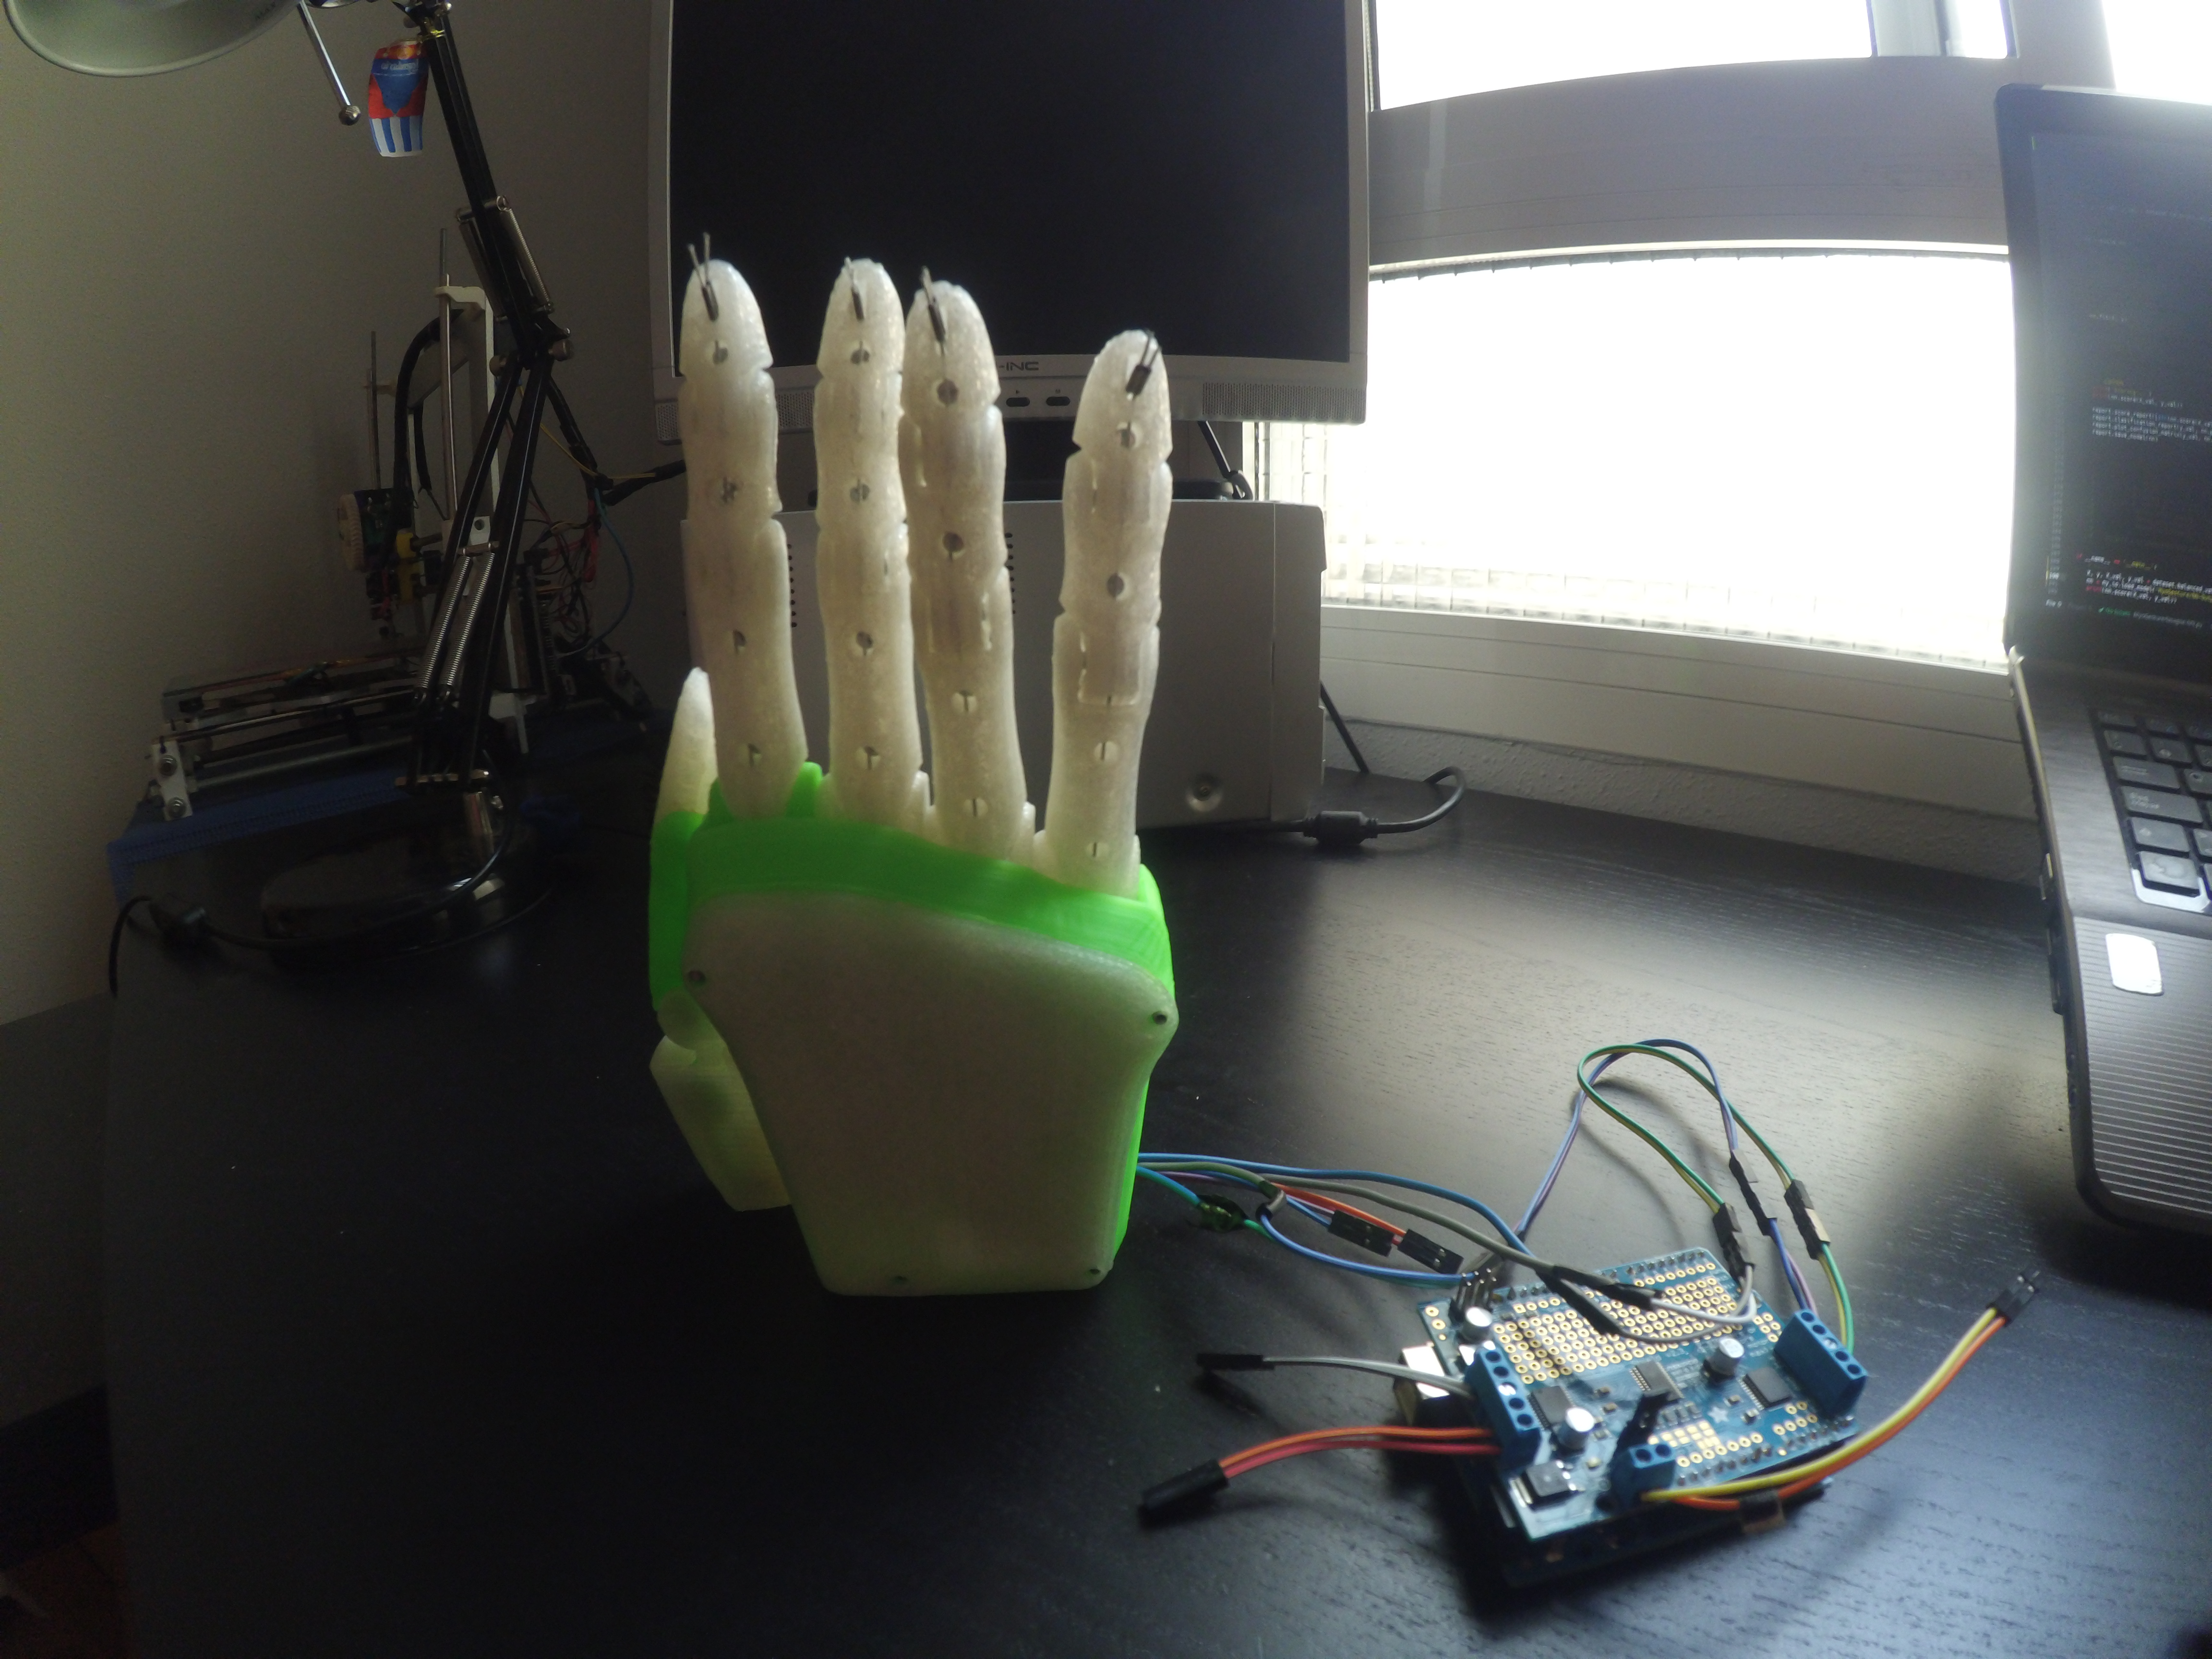
\includegraphics[width=1\textwidth]{Chapter2/dorsal}
  \caption{Vista del dorsal de la prótesis terminada}
\label{fig:dorsal}
\end{figure}


\begin{figure}[htp]
  \centering
    \includegraphics[width=1\textwidth]{Chapter2/palma}
  \caption{Vista del palmar de la prótesis terminada}
\label{fig:palmar}
\end{figure}


\subsection{Desarrollo de la prótesis}

En el anexo \ref{presupuestoProyecto} se especifica los materiales utilizados tanto para la creación de la prótesis como la parte de la electrónica que la controlará.


Los modelos 3D de la prótesis Dextrus \ref{fig:dorsal} \ref{fig:palmar} pueden descargarse en \cite{openbionics-downloads} y las instrucciones del montaje en
\cite{dextrus-instructions}. El mayor problema ha sido encontrar ciertos materiales, en concreto: tornillería de
métrica dos o inferior (tienda de modelismo especializado), los cables que emulan los tendones (hilos métalicos de
pesca), las virolas para unir los dos extremos de los cables (material de pesca) y clavijas o tarugos de metal, que
son las piezas que se introducen en los rodamientos (este ha sido el componente más difícil de encontrar ya que
el modelo de la prótesis requiere longitudes de este componente muy determinadas -se pueden consultar en el anexo
\ref{presupuestoProyecto} -, para conseguirlo se ha tenido que cortar y limar destornilladores de 3mm de anchura a mano).







\subsection{Componentes electrónicos}

La electrónica consiste básicamente en el controlador de motores, que controla el movimiento de los motores de la prótesis, y el Arduino, que se encarga de cuándo deben moverse los motores. Para poder alimentar tanto los
componentes electrónicos como los motores que están dentro de la prótesis, se ha utilizado para el entorno de pruebas una fuente de alimentación de PC (fuera de este entorno la fuente sería sustituida por una batería
recargable, pero esto queda fuera del trabajo y se propone como futuras mejoras).
%TODO añadir batería de a trabajo futuro.

La alimentación a todos los componentes se realiza mediante el controlador de motores, que recibe una tensión de 12V desde la fuente. Para utilizar los cables de esa intensidad \cite{power-pc} de deben seguir los siguientes pasos \textbf{siempre con la fuente desconectada de la red eléctrica}:

\begin{itemize}
\item Crear un puente entre el pin PS\_ON y cualquiera de los cables de toma de tierra (Ver figura \ref{fig:atx-colors} para comprobar los colores).

\item Sacar los cables de 12V de tensión (color amarillo). Se puede usar regletas y cables macho-hembra para facilitar el proceso de conexión y desconexión como se muestra en la figura \ref{fig:mi-fuente}.

\end{itemize}

\begin{figure}[htp]
  \centering
    \includegraphics[width=0.6\textwidth]{Chapter2/atx-colors}
  \caption{Información sobre los pines de una fuente de alimentación ATX. Imagen extraida de wikipedia.org}
\label{fig:atx-colors}
\end{figure}



\newpage
\subsection{Entorno de pruebas}

En las figuras \ref{fig:mi-fuente} y \ref{fig:mi-prótesis} se puede observar los componentes que se utilizarán para realizar las pruebas reales con el modelo de clasificación desarrollado a lo largo del proyecto.

\begin{figure}[htp]
  \centering
    \includegraphics[width=0.85\textwidth]{Chapter2/mi-fuente}
  \caption{Fuente de alimentación preparada para utilizar 12V.}
\label{fig:mi-fuente}
\end{figure}

\begin{figure}[htp]
  \centering
    \includegraphics[width=0.85\textwidth]{Chapter2/mi-protesis}
  \caption{Arduino con el controlador de motores acoplado junto con la prótesis y sus componentes al descubierto.}
\label{fig:mi-prótesis}
\end{figure}
